%Questo modello fa più schifo di quelli di prima, dropout scartato
\begin{table}[H]
    \centering
	\begin{tabular}{lcccc}
	\textbf{Layer Type} & \textbf{Layer Config} & \textbf{Activation}  & \textbf{Output} & \textbf{Params}\\ \hline
	\conv	& \convKSF{5}{1}{5}	& relu		& \texttt{144,256,5} 	& \texttt{380}\\
	\pool	& \poolN				&	/		& \texttt{72,128,8}		& 0	\\
	\conv	& \convKSF{5}{1}{8}	& relu		& \texttt{72,128,8} 		& \texttt{1008}\\
	\pool	& \poolN				&	/		& \texttt{36,64,12}		& 0	\\	
	\conv	& \convKSF{3}{1}{12}	& relu		& \texttt{36,64,12} 		& \texttt{876}\\
	\pool	& \poolN				&	/		& \texttt{18,32,15} 		& 0	\\
	\conv	& \convKSF{3}{1}{15}	& relu		& \texttt{18,32,15} 		& \texttt{1635}\\
	\pool	& \poolN				&	/		& \texttt{9,16,18}		& 0	\\
	\conv	& \convKSF{3}{1}{18}	& relu		& \texttt{9,16,18} 		& \texttt{2448}\\
	\drop	& \dropR{0.75}		&	/		& \texttt{9,16,18}		& 0\\
	
	\flt		& /					& /			& \texttt{2592}			& \texttt{0}\\
	\dns		& \dnsP{64}			& relu		& \texttt{64}			& \texttt{165952}\\
	\drop	& \dropR{0.75}		&	/		& \texttt{64}			& 0\\
	\dns		& \dnsP{6}			& softmax	& \texttt{6}				& \texttt{390}\\
	\end{tabular}
	%Total params: 172,689
	%Trainable params: 172,689
	%Non-trainable params: 0
\end{table}


\begin{table}[H]
	\centering
	\begin{tabular}{lc}
	\textbf{Param} & \textbf{Value}\\ \hline
	Batch Size 	& 32 \\
	Optimizer 	& Adam \\
	Base lr		& 0.001 \\
	Epochs		& 20 \\
	\end{tabular}
\end{table}


\begin{figure}[H]
	\begin{center}
	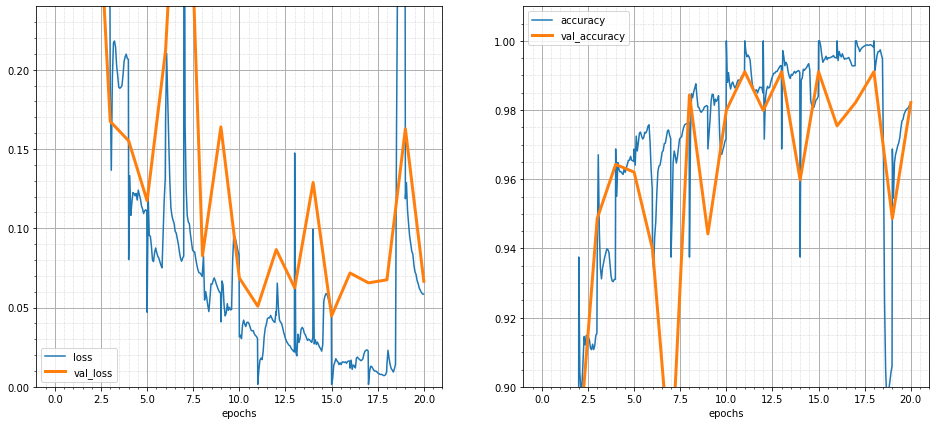
\includegraphics[width=\linewidth]{Immagini/conv-drop-pool-1}
	\caption{Graph of the first run}
	\end{center}
\end{figure}
\begin{table}[H]
	\centering
	\begin{tabular}{cccccc}
		\textbf{Run} &\textbf{Loss}&\textbf{V.Loss} &\textbf{Acc.}&\textbf{V.Acc.}&\textbf{$\Delta$ Acc.} \\ \hline
		1   & 0.0582    & 0.0666    & 0.9817    & 0.9821    & -0.0004\\
		2   & 0.0063    & 0.0269    & 0.9987    & 0.9933    & 0.0054\\
		3   & 0.1172    & 0.0615    & 0.9654    & 0.9866    & -0.0212\\
		\textbf{Avg} & \textbf{0.0606}    & \textbf{0.0517}    & \textbf{0.9820}    & \textbf{0.9873}    & \textbf{-0.0054}
	\end{tabular}
\end{table}

The next iteration of the model added dropout regularization after the two layers with the most trainable parameters. The desired goal was to chip away another bit off the difference between the training set and the validation set.\\
While this definitely worked, as seen by the negative average $\Delta$ accuracy, it came with a slight reduction in the overall validation accuracy.